\documentclass[12pt]{article}
\usepackage[utf8]{inputenc}
\usepackage[english,russian]{babel}
\usepackage{amsmath}
\usepackage{amssymb}
\usepackage{geometry,indentfirst,color}
\usepackage[pdftex]{graphicx}
\usepackage{sidecap}
\geometry{top=0.5cm} %поле сверху
\geometry{bottom=0.5cm} %поле снизу
\geometry{left=1.5cm} %поле справа
\geometry{right=1.5cm}
\usepackage{wrapfig}
\usepackage{epigraph}
%\pagestyle{empty}
\DeclareGraphicsExtensions{.pdf,.png,.jpg}
\DeclareMathOperator{\Tr}{Tr}
\setlength{\textheight}{24cm}\newcounter{nnn}\setlength{\topmargin}{-20mm}
\begin{document}
\begin{flushleft}
\parbox[t][0pt]{0.2\textwidth}
{
{%\centering
\vspace{0\baselineskip}

\includegraphics[scale=1.5]{klsh_logo_mod.pdf}\par
}
}
\end{flushleft}
\newcommand{\klshyear}{2025}
\hfill
\parbox[t][0pt]{0.80\textwidth}
{
{\centering
\vspace{-1.5\baselineskip}
\begin{flushright}
{\Huge Правила ФМТ}\\
{Красноярская Летняя Школа $\klshyear$}\par
По всем вопросам: {\it  Роберт Гринштейн, Борис Демешев}
\end{flushright}
}
}
\vspace{4\baselineskip}

\section*{Общие положения}
Физико-математический турнир (ФМТ)~--- один из самых первых и уважаемых турниров Красноярской Летней Школы, сочетающий в себе как дух здоровой соревновательности, так и множество возможностей узнать что-то новое (и не только для школьников). Основная часть турнира~--- 6 туров, которые пройдут в течение сезона. Встреча команд в первом туре определяется жеребьёвкой. В последний день сезона проходит свалка~--- необычный тур, который во многом уравнивает шансы команд выйти в финалисты и проводится по отдельным правилам. Наконец, проводятся финал и суперфинал, в которых определяются три команды-победительницы, награждаемые ценными призами.

Правила турнира, стратегии и задачи не раз менялись за годы работы КЛШ, но главное оставалось неизменным: на турнире всегда в почёте честность, красивая игра, здоровая соревновательность и воля к победе.

\section*{Тест-драйв ФМТ}
Тест-драйв ФМТ проводится в первый день летней школы и выступает в роли знакомства команд впервые (или вновь) с форматом физико-математического турнира. В рамках этого тура будут предложены 4 задачи (подробнее в \textbf{Основной этап}). Сразу стоит отметить, что этап \textbf{Обмена ударами} \textit{не проводится}!  По результатам этого тура производится жеребьевка команд на 1-й тур летней школы, причем результат этого тура домнажается на коэффициент $0.5$, что уменьшает его вес в рамках всех туров ФМТ. Жеребьевка повлияет только на изначальное распределение команд для дальнейшей захватывающей и интересной игры в рамках последующих 6 турах ФМТ!

\section*{Основной тур}
Основной тур состоит из двух этапов: \textsl{основной этап} и этапа \textsl{обмена ударами}. Каждая КЛШ-команда\footnote{Под КЛШ-командой понимается команда, обозначаемая буковкой греческого алфавитика.} выставляет на основной тур до четырёх человек (меньше четырёх можно, но не желательно), которые и составляют ФМТ-команду (далее просто ``команда'')\footnote{Состав команды в каждом туре может быть разным.}. Каждая КЛШ-команда может выставить произвольное число вольных стрелков (см.~ниже). К началу тура команда должна явиться вовремя, при себе имея {\bf два} идентичных экземпляра обменной задачи на бумажном носителе.

\subsection*{Основной этап}
Основной этап длится 20 минут. Команды получают одинаковые комплекты из четырёх задач: как правило, две по физике (``простая'' и ``сложная'') и две по математике (аналогично). Подумайте над тем, как распределить ваши силы при решении задач. Для дальнейшего обсуждения представим, что в туре участвуют команды ``кси'' ($\xi$) и ``дзета'' ($\zeta$).

\noindent{\bf Заявка}. Для любой задачи первым возможным действием команды является {\bf заявка}. Если команда $\xi$ считает, что решила задачу, то один из членов команды громко произносит: \textsl{Команда $\xi$ заявляет задачу номер ...}. В этот момент судьи в обязательном порядке должны опросить вольных стрелков и принять от них решение заявленной задачи в письменном виде. Затем судья сразу же просит представителя команды-заявительницы ($\xi$ в нашем случае) сообщить ответ и фиксирует его на доске. Будьте внимательны: если заявленный ответ неверен, то это лишает команду возможности получить полный балл за задачу.

Второе по регламенту действие, которое команда должна совершить~--- {\bf доклад}. Докладчик от команды $\xi$ выходит к доске для доклада, при этом команда $\zeta$ обязана выставить оппонента. Оппоненту будет предоставлено специальное время, когда он сможет задать вопросы докладчику, обеспечивающие понимание изложенного докладчиком решения \iffalse(по смыслу вопросы нужны, чтобы прояснить решение оппоненту)\fi и сформулировать замечания к изложенному решению\footnote{Обратите внимание, что вопрос и замечание~--- это не одно и то же. Оппонент зарабатывает свои очки за замечения, но не за вопросы. Будьте внимательны и не делайте замечаний, когда судья просит вопросы.}. Докладчик излагает решение, при этом можно пользоваться собственными записями, сделанными во время работы за столом.

Третье по регламенту действие~--- \textbf{оппонирование}. Судья спрашивает оппонента, всё ли ему понятно в изложенном решении, и если оппоненту что-то осталось непонятным, оппонент имеет возможность задать вопросы для понимания. Далее оппонент может высказать свои замечания по решению (даже если он был согласен с решением): если замечания были сделаны по существу и действительно раскрывают пробелы и ошибки в решении, то судьи дадут команде $\zeta$ очки за оппонирование.

После доклада и оппонирования судьи принимают решение о том, снимается данная задача или нет. Задача может быть снята, если судьи сочли, что основные идеи решения были изложены. Если задача не снимается судьями, то происходит

\noindent\textbf{Переход подачи}. Это означает, что задача не решена, не снята и команды продолжают её решение. Однако безусловное право заявки переходит теперь к команде оппонента ($\zeta$ в нашем примере) и встреча продолжается по регулярным правилам.

\noindent\textbf{Результат заявки}. Возможны следующие варианты исхода событий:
\begin{list}{\arabic{nnn})}{\usecounter{nnn}\leftmargin=6mm \labelwidth=5mm \topsep=0mm \labelsep=2mm \itemsep=1pt \parsep=0mm \itemindent=10pt}
\item Команда-заявитель получает \textbf{3 балла} если:
	\begin{itemize}
		\item Правильный заявленный ответ; 
		Правильное решение;
		Правильный итоговый ответ.
	\end{itemize}

\item Команда-заявитель получает \textbf{2 балла} если
	\begin{itemize}
		\item Неправильный заявленный ответ;
	Правильное решение;
	Правильный итоговый ответ.
	\item Правильный заявленный ответ;
	Несущественная ошибка в счёте;
	Правильный итоговый ответ.
	\end{itemize}

\item Команда-заявитель получает \text{1 балл} если
	\begin{itemize}
		\item Заявленный и итоговый ответы неправильные (вычислительная ошибка)
	Правильная модель
	\item Недостаточное решение (например, не доказана единственность решения), однако ответ верный
	\item Существуют задачи, в которых 1 балл можно получить в некоторых особых случаях. Об этих задачах и случаях получения будет сказано на разборах
	\end{itemize}

\item Команда-заявитель получает \text{0 баллов} если
	\begin{itemize}
		\item Остальные случаи (все неправильно) 
	\end{itemize}
\end{list}

\textbf{Оппонент} может получить максимум \textbf{1 балл}, когда делает замечание.

За угаданный ответ или ответ без объяснения решения школьник получает \textbf{0 баллов} и переход подачи. 
Даже если получен правильный ответ, но само решение неверно, школьник получает \textbf{0 баллов} и задача переходит к сопернику.

Следует подчеркнуть, что число переходов подачи по каждой задаче формально ничем не ограничено. Решение каждой задачи принимается и оценивается независимо (и может быть, параллельно во времени) друг от друга.

\noindent{\bf Вольные стрелки}: Каждая КЛШ-команда вправе выставить на встречу любое количество вольных стрелков из состава КЛШ-команды. Чтобы вольные стрелки заработали очки, они должны в {\bf письменном} виде оформить решение задачи и передать его судейской бригаде {\bf до} того, как задача (точнее, ответ на задачу) будет объявлен. За каждую задачу стрелки могут заработать до двух очков (их решения не оппонируются). Стрелки могут заявлять любую из четырёх задач, но в итоге стрелки смогут принести команде {\bf не более трех} очков\footnote{Вам кажется, что это не очень весомо? В турнире 4 задачи, грубо говоря, это 12 очков, команды при равной игре зарабатывают по 6 очков. А стрелки могут принести к этим очкам дополнительно три, то есть 50\,\%.}.

\subsection*{Обмен ударами}
По окончании основного этапа наступает этап обмена ударами; его продолжительность составляет 10 минут. Каждая команда подготовила {\bf две идентичных} копии своей обменной задачи (одна --- судьям, вторая --- для соперников). Копии должны быть правильно подписаны, вроде ``Команде $\zeta$ от команды $\xi$''. Командам даётся 10 минут на решение задачи соперника. Первой докладывать задачу оппонента попросят команду, которая по итогам I эпапа встречи имеет больше баллов.

{\bf Обменная задача}: Ох, сколько команд страдает из-за того, что они неправильно готовят обменную задачу! Прочтите эту часть и не наступайте на их грабли. Итак, что такое хорошая обменная задача? 
\begin{enumerate}
\item Это должна быть задача по {\bf физике или математике}. Хорошо, если задача красивая, с интересной идеей\footnote{Хоть это и не обязательно, но мы очень любим глубокие, интересные задачи, и регулярно дарим призы за красоту обменных задач.}. 

\item Но самое главное, она должна быть {\bf хорошо сформулирована}. Если вы берёте задачу из книжки, убедитесь, что вы не упустили чего-то важного в условии. Даже если задача взята из книжки, её формулировка может быть недостаточно строгой и ясной для обменного эпапа ФМТ (например, условие имеет смысл только в контексте этой книжки). Покажите свою обменную задачу вожатым: понятна ли им формулировка? 

\item Важно понять: судить будут то, что {\bf написано}, а не то, что вы имели в виду. Если условие допускает двусмысленную трактовку, то соперники вправе решать задачу в более лёгкой форме\footnote{Суперфинал ФМТ-2010, команда $o$ спрашивает: для какой функции $f(x)$ числа $x$, $f(x)$ и $f(f(x))$ не могут быть сторонами треугольника ни при каких $x$? Ответ команды $\sigma$: $f(x) = -x$, для любого $x$ одна из сторон отрицательна. Команда $o$ забыла написать, что функция $f(x)$ должна быть строго положительна, имелось в виду $f(x) = x^2 + 1$.}. 

\item Обратите внимание, что задача не должна выходить за пределы школьной программы. В противном случае судьи могут попросить вас вывести внешкольные утверждения, на которые вы опирались в решении, в те же три минуты вашего доклада. Если вы сомневаетесь, проходит ли ваша задача по этому требованию, поговорите с одним из судей ФМТ\footnote{Только пусть это будет не вожатый вашей команды-соперника, иначе всё пропало!}.

\item Наконец, хочется спросить, что вы думаете о просьбе продолжить последовательность $0$, $1$, $2$, $\ldots$? Если вам кажется, что это хорошая задача, то ваш оппонент ответит: следующий член последовательности --- <<Гарри Поттер>>, и получит полный балл за решение.

\item Если же ваша команда захочет заявить задачу в духе <<На какие 100 цифр оканчивается число 98!~?>>, то такую задачу судьи вправе \textbf{забраковать}. Как и в любом другом соревновании, многие правила и законы основаны на обычной этике происходящего. Таким образом, настоятельно вам советуем  {\bf не давать подобных задач}.

\item Три минуты --- действительно серьёзное ограничение по времени. Оно было введено для того, чтобы <<оживить>> второй эпап, стимулировать команды не давать <<гробы>>. Для того, чтобы задача была докладываемой за три минуты, интересной и сложной для соперника, тебе может понадобиться помощь сотрудников НТН. Пожалуйста, не стесняйся подойти к любому сотруднику направления и посоветоваться, хороша ли ваша задача, хороша ли формулировка. Наши сотрудники дружелюбны, приветливы и всегда тебе помогут.
\end{enumerate}
{\bf Доклад задачи соперника}: Расслабьтесь, это самая спокойная часть игры. Если вам кажется, что вы что-то поняли в задаче оппонента, вы можете выходить к доске её решать. Заявлять ответ не нужно\footnote{Вы уже догадались, что это значит, что вы можете дорешивать задачу у доски? Только нужно это делать так, чтобы судьи не догадались: если судья посчитает, что вы не знаете, что делать дальше, и топчетесь на месте, доклад прервут.} и нет оппонирования со стороны команды соперника. Вердикт о правильности или неправильности решения выносит только судейская бригада. За решение вы получаете до трех баллов.

{\bf Доклад своей задачи}: Пожалуй, это самая сложная часть эпапа\footnote{Только если у вас плохая обменная задача.}. Решение своей задачи нужно доложить {\bf за три минуты, включая вопросы судей}. ``Как!? --- воскликнете вы. --- Времени в обрез, а нам ещё будут вопросы задавать? Это нечестно!'' Не совсем. Судьи требуют лишь, чтобы ваше решение было {\bf полным}: без пробелов, с чётким пониманием происходящего. Вопросы будут задавать лишь в случае, если ваш доклад содержит серьёзные пробелы. {\bf Отчет времени} начинается с момента прочитки условия задачи докладчиком. Ее решение нужно рассказывать полностью по памяти, все вычисления нужно проделывать на доске в процессе доклада. Важно: решение может докладывать {\bf любой} член команды по желанию самой команды.

Если вы не уложились в предоставленное время или ваше решение просто неверное, то судьи могут оштрафовать команду на один или два балла. Также не стоит рассказывать решение быстро наговаривая его, словно вы Eminem, исполняющий "Rap God". Судьи вправе сначала {\bf оставновить} вас, попросив рассказывать решение помедленнее, а при повторе нарушения вовсе {\bf оштрафовать} на один балл.

\subsection*{Штрафы}
В течение тура команда может не только зарабатывать очки, но и терять их. За опоздание, громкое поведение, неителлигентные споры с судьями может быть наложен дисциплинарный штраф до трех баллов. Также нужно помнить про штраф за незнание собственной обменной задачи: (до трех баллов). Сколько трагедий\footnote{Мы боимся, что и ещё будут\ldots} было в летней школе из-за незнания решения собственной задачи! Главный источник трагедий~--- ошибки при переписывании условия из задачника (и вообще~--- из источника) на бумагу. Школьники склонны украшать текст деталями, связанными с реалиями летней школы; это чревато потерей важных мелочей. Другой источник ошибок~--- плохое понимание условия задачи. Например, в условии говорится о некотором свойстве окружности, а школьники пишут про круг. В результате они думают, что располагают решением своей задачи, но на самом деле предложенная задача с кругом вместо окружности может вообще не иметь решения.

\subsection*{Подписание протоколов и апелляция}
Когда тур подошёл к концу (окончился этап обмена ударами), команды ставят свои подписи в протоколе встречи. Если команда не согласна с {\bf действиями судей} на одном из этапов (или в обоих), то вместо подписи капитан команды должен написать слово ``\textsl{апелляция}''\footnote{Пишите это слово грамотно, иначе судьи могут вредничать.}. После этого в течение {\bf одного часа} команда должна предоставить главному судье ФМТ суть своих претензий в письменном виде. Для рассмотрения этих претензий будет создана апелляционная комиссия; её решения являются окончательными, а в состав входят наиболее квалифицированные судьи, не принимавшие участия в судействе оспариваемой встречи. Если комиссия решит, что претензии обоснованы, то счёт той части тура (основного времени или обмена ударами), которая была оспорена, становится равным $0:0$. Пожалуйста, не относитесь к апелляции как к возможности изменить итог любой встречи. Подавайте её лишь в том случае, когда вы уверены в своих претензиях, иначе это будет лишь пустая трата времени для всех.

\subsection*{Разбор задач}
После каждого тура судейская бригада организует разбор задач основного этапа. ``Да ну! --- зевнёте вы, --- Мы устали, хотим полежать.'' Благородное желание. Но дело в том, что некоторые задачи, которые мы даём на основном этапе, могут повториться в следующих турах в несколько изменённом (обычно усложнённом) виде\footnote{Так называемые <<цепные>> задачи.}. Узнав каноническое решение от судей, вы сильно повышаете свои шансы на успех в следующих турах.

\section*{Между основными турами}
Обменные задачи, которые были использованы в прошлых турах, публикуются на столовой. Поэтому не стоит использовать одну и ту же обменную задачу из тура в тур. В течение всей школы мы ведём турнирную таблицу, стараясь делать так, чтобы между собой играли близкие по силе команды, при этом не допускаем, чтобы две команды встречались дважды. Положение в таблице определяется суммой очков, набранных командой за прошедшие туры: за победу команда получает два очка турнирной таблицы, за ничью --- одно очко\footnote{Кроме того, мы учитываем баллы, набранные в туре за решение задач, чтобы снять вырождение при сортировке команд. Спросите судей, если вам это интересно.}. По итогам всех основных туров каждая команда получает от 0 до 23 {\bf финальных очков}, равное числу команд, сыгравших хуже данной.

\section*{Игровой тур}
В этом сезоне летней школы также будет проводится тур, разительно отличачющийся от остальных классических туров ФМТ. В рамках этого тура командам будет предложена \textbf{логическая игра}, правила которой вы узнаете {\it накануне} тура. Судьи перед началом тура представят вам пример {\it разыгровки} по правилам игры. Также, как и на {\bf тест-драйве}, обменную задачу готовить \textbf{не надо} (ура!). Сначала вам (игроку из вашей команды) предстоят баталии с оппонентом (игроком из другой команды). По результатам сражения, будет выставлен счет встречи в рамках каждой пары {\it дуэлянтов}. Также, как и в \textbf{}{Основном этапе}, результат по каждой паре будет суммироваться. После этого игра переход к этапу \textbf{Стенка на стенку}.
\subsection*{Стенка на стенку}
В рамках данного этапа вы играете в ту же самую игру, но теперь уже поле сражения смещается на судейскую доску. Вам предстоит командой отвечать на ходы противника. Результат этого тура также пойдет в счет встречи.

Вес \textbf{игрового тура} в рамках ФМТ \textbf{сохраняется}, то есть он также важен как и остальные туры.
\section*{Свалка}
Свалка проходит в последний день КЛШ и напоминает основной этап регулярного тура ФМТ. Главное: команда борется не против одного соперника, а против {\bf хронометра}. Каждая команда получает 4 задачи. Команда решает задачи так, чтобы судья видел ход решения (а соперники не слышали!) и заявляет свой ответ на специальном бланке. Судья фиксирует время заявки и число очков за решение: ноль, один, два или три. Заявлять задачи на свалке можно в произвольном порядке.

В процессе тура мы обрабатываем данные:
\begin{enumerate}
	\item За каждую задачу команда может получить до 1200 штрафных секунд. Число штрафных секунд за задачу определяется следующим образом: если задача решена на 0 баллов, команда получает 1200 штрафных секунд; если задача решена на 1 балл, команда получает штрафных секунд столько, сколько секунд прошло с момента начала свалки до момента заявки задачи; если задача решена на 2 балла, команда получает {\bf половину} от числа секунд, прошедших с момента начала свалки до момента заявки задачи\footnote{Лучше решить задачу на два балла за 20 минут, чем на один балл за 1 минуту.}.;
	\item Штрафные секунды по задачам суммируются, таким образом команда может набрать до 4800 штрафных секунд;
	\item Мы сортируем команды по возрастанию числа штрафных секунд, и каждая команда получает столько {\bf финальных очков}, сколько команд выступило хуже неё (от 0 до 23).
\end{enumerate}

\section*{Финал и суперфинал}
Как вы помните, за основные туры и за свалку можно было набрать от $0$ до $23$ {\bf финальных очков}. Сложим эти очки за основные туры и за свалку. По этой сумме финальных очков мы определяем, какие команды сойдутся в финале и суперфинале: IV и III команды сразятся в финале, а II и I команды будут бороться в суперфинале.

Суперфинал и финал похожи на обычные туры ФМТ за следующими исключениями:
\begin{enumerate}
\item Нет вольных стрелков.
\item Сложные задачи.
\item Судейская бригада {\bf случайным образом} определяет, кто из членов команды будет докладывать решение своей задачи на обмене ударами. Таким образом, решение обменной задачи должны знать {\bf все} участники\footnote{Забыл! Можно выучить не всем и понадеяться на удачу!}.
\end{enumerate}

\section*{Блок-схема туров ФМТ}
Этот рисунок будет вашим помощником в сезоне. С помощью этой картинки вы будете понимать что нужно сделать к текущему туру, что вас ожидает и т.д. и т.п.
\begin{figure}[h!]
	\centering{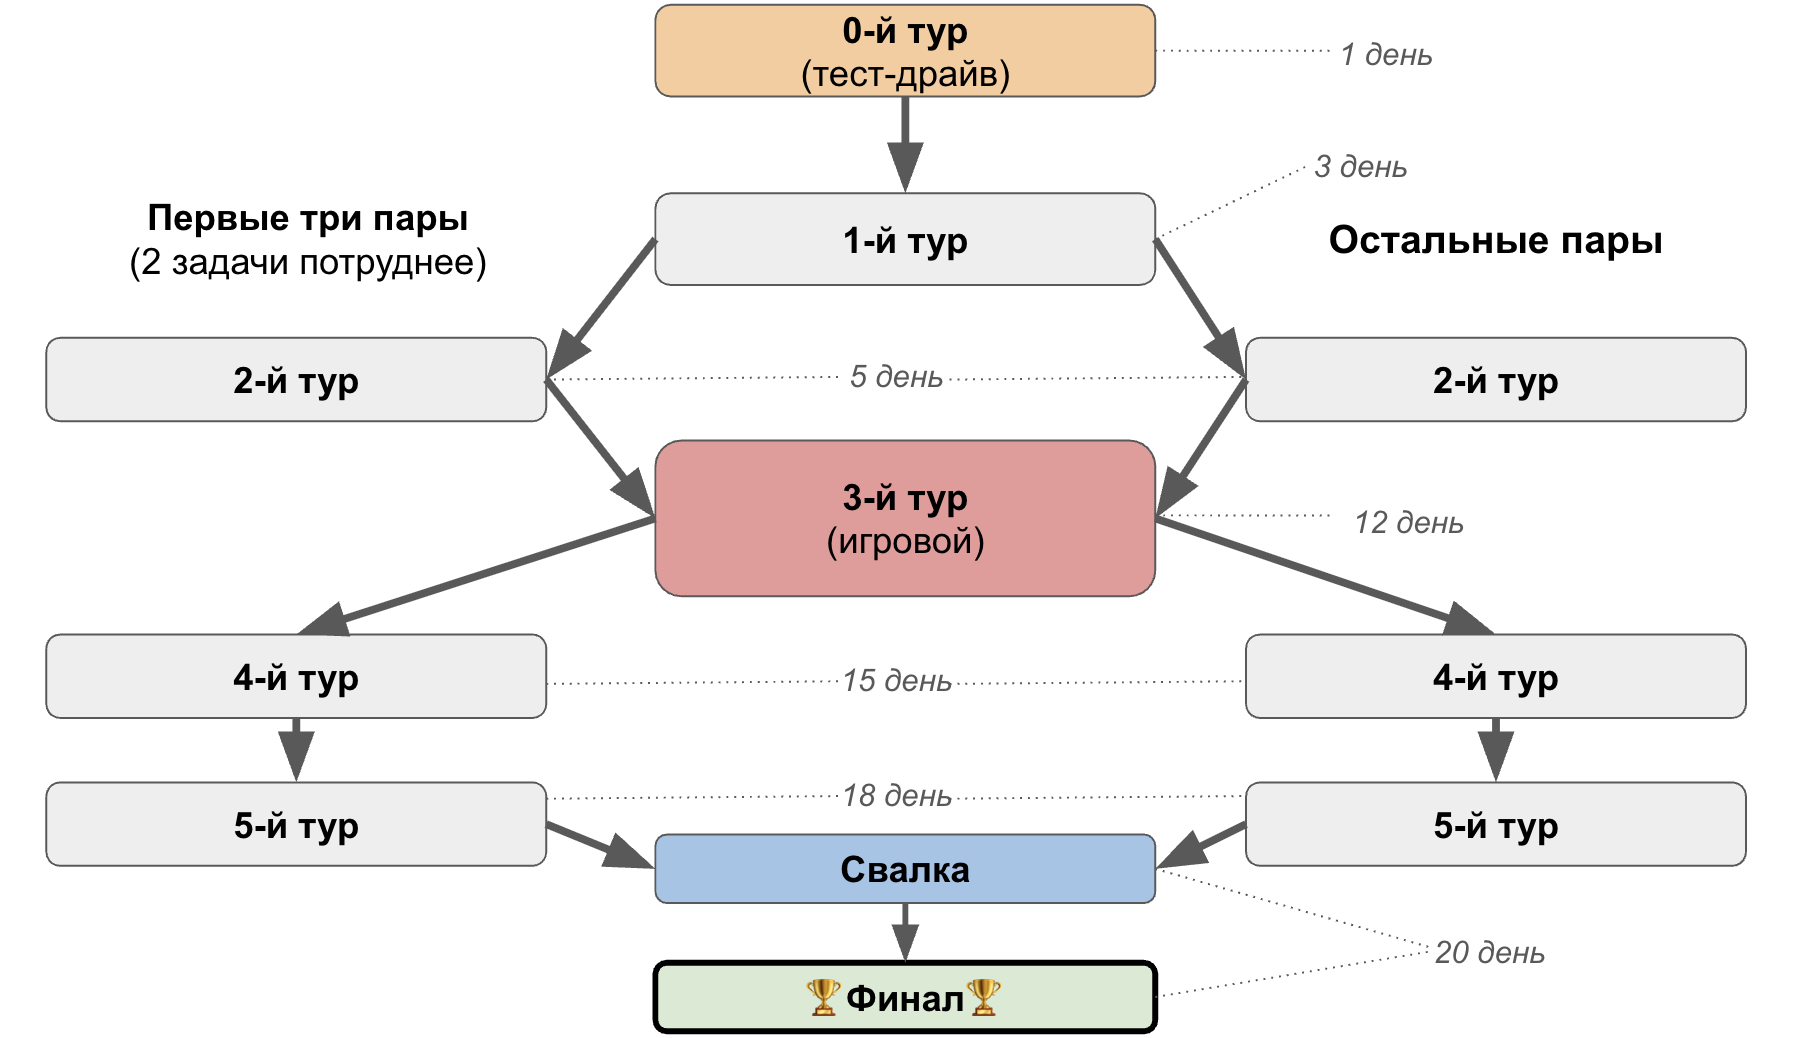
\includegraphics[scale=0.5]{scheme.png}}
	\caption{На блок-схеме серым обозначены \textbf{основные туры}, а цветным - \textbf{примечательные}.}
\end{figure}

\hrule
\vspace{6pt}
\noindent Судьи ФМТ, к которым можно обращаться по поводу {\bf обменных задач}
\begin{center}
	{\it Роберт Гринштейн, Боря Демешев, Ваня Адо, Сережа Ламзин, Рома Лисин, Ян Шапиро, Влада Синицына, Егор Лунев} и остальные сотрудники НТН
\end{center}

\end{document}